%  The AAU Poster Theme.
%  2013-05-08 v. 1.1.0
%  Copyright 2013 by Jesper Kjær Nielsen <jkn@es.aau.dk>
%
%  This is free software: you can redistribute it and/or modify
%  it under the terms of the GNU General Public License as published by
%  the Free Software Foundation, either version 3 of the License, or
%  (at your option) any later version.
%
%  This is distributed in the hope that it will be useful,
%  but WITHOUT ANY WARRANTY; without even the implied warranty of
%  MERCHANTABILITY or FITNESS FOR A PARTICULAR PURPOSE.  See the
%  GNU General Public License for more details.
%
%  You can find the GNU General Public License at <http://www.gnu.org/licenses/>.
\documentclass[a0paper,portrait]{baposter}
\usepackage{relsize}	
\usepackage{blindtext}
\usepackage[utf8]{inputenc}
\usepackage{sidecap}
% Make latex understand and use the typographic
% rules of the language used in the document.
\usepackage[english]{babel}
% Use the vector font Latin Modern which is going
% to be the default font in latex in the future.
\usepackage{helvet}
% Change the default font family from roman to sans serif
\renewcommand{\familydefault}{\sfdefault} % for text
\usepackage[helvet]{sfmath} % for math
% Choose the font encoding
\usepackage[T1]{fontenc}

%%%%%%%%%%%%%%%%%%%%%%%%%%%%%%%%%%%%%%%%%%%%%%%%
% Graphics and Tables
% http://en.wikibooks.org/wiki/LaTeX/Importing_Graphics
% http://en.wikibooks.org/wiki/LaTeX/Tables
% http://pgfplots.sourceforge.net/
%%%%%%%%%%%%%%%%%%%%%%%%%%%%%%%%%%%%%%%%%%%%%%%%
% You cannot use floats in the baposter theme.
% We therefore load the caption package which provides
% the command \captionof
% Set up how figure and table captions are displayed

\usepackage{caption}
\captionsetup{
  font=small,% set font size to footnotesize
  labelfont=bf % bold label (e.g., Figure 3.2) font
}
% Make the standard latex tables look so much better
\usepackage{array,booktabs}
% For creating beautiful plots
\usepackage{pgfplots}

%%%%%%%%%%%%%%%%%%%%%%%%%%%%%%%%%%%%%%%%%%%%%%%%
% Mathematics
% http://en.wikibooks.org/wiki/LaTeX/Mathematics
%%%%%%%%%%%%%%%%%%%%%%%%%%%%%%%%%%%%%%%%%%%%%%%%
% Defines new environments such as equation,
% align and split 
\usepackage{amsmath}
% Adds new math symbols
\usepackage{amssymb}

%%%%%%%%%%%%%%%%%%%%%%%%%%%%%%%%%%%%%%%%%%%%%%%%
% Colours
% http://en.wikibooks.org/wiki/LaTeX/Colors
%%%%%%%%%%%%%%%%%%%%%%%%%%%%%%%%%%%%%%%%%%%%%%%%
\selectcolormodel{RGB}
% define the three aau colors
\definecolor{aaublue1}{RGB}{33,26,82}% dark blue
\definecolor{aaublue2}{RGB}{113,109,143} % light blue
\definecolor{aaublue3}{RGB}{194,193,204} % lighter blue
\definecolor{luered}{RGB}{147,57,73} % lueneburg red
\definecolor{upbblue}{RGB}{33,26,82}% not yet the right blue
\definecolor{skyblue}{rgb}{0.53, 0.81, 0.92}
\definecolor{orangew}{rgb}{1.0, 0.65, 0.0}
\definecolor{deepskyblue}{rgb}{0.0, 0.75, 1.0}
\definecolor{orangec}{rgb}{1.0, 0.5, 0.0}

\usetikzlibrary{decorations.pathmorphing,calc,shapes,arrows,shapes.geometric,patterns,shadows,arrows.meta,fadings}


%%%%%%%%%%%%%%%%%%%%%%%%%%%%%%%%%%%%%%%%%%%%%%%%
% Lists
% http://en.wikibooks.org/wiki/LaTeX/List_Structures
%%%%%%%%%%%%%%%%%%%%%%%%%%%%%%%%%%%%%%%%%%%%%%%%
% Easier configuration of lists
\usepackage{enumitem}
%configure itemize
\setlist{%
  topsep=0pt,% set space before and after list
  noitemsep,% remove space between items
  labelindent=\parindent,% set the label indentation to the paragraph indentation
  leftmargin=*,% remove the left margin
  font=\color{aaublue1}\normalfont, %set the colour of all bullets, numbers and descriptions to aaublue1
}
% use set<itemize,enumerate,description> if you have an older latex distribution
\setitemize[1]{label={\raise1.25pt\hbox{$\blacktriangleright$}}}
\setitemize[2]{label={\scriptsize\raise1.25pt\hbox{$\blacktriangleright$}}}
\setitemize[3]{label={\raise1.25pt\hbox{$\star$}}}
\setitemize[4]{label={-}}


%%%%%%%%%%%%%%%%%%%%%%%%%%%%%%%%%%%%%%%%%%%%%%%%
% Misc
%%%%%%%%%%%%%%%%%%%%%%%%%%%%%%%%%%%%%%%%%%%%%%%%
% change/remove some names
\addto{\captionsenglish}{
  %remove the title of the bibliograhpy
  \renewcommand{\refname}{\vspace{-0.7em}}
  %change Figure to Fig. in figure captions
  \renewcommand{\figurename}{Fig.}
}
% create links
\usepackage{url}
%note that the hyperref package is currently incompatible with the baposter class

%%%%%%%%%%%%%%%%%%%%%%%%%%%%%%%%%%%%%%%%%%%%%%%%
% Macros
%%%%%%%%%%%%%%%%%%%%%%%%%%%%%%%%%%%%%%%%%%%%%%%%
\newcommand{\alert}[1]{{\color{aaublue1}#1}}


%%%%%%%%%%%%%%%%%%%%%%%%%%%%%%%%%%%%%%%%%%%%%%%%
% Document Start 
%%%%%%%%%%%%%%%%%%%%%%%%%%%%%%%%%%%%%%%%%%%%%%%%
\begin{document}
%%%%%%%%%%%%%%%%%%%%%%%%%%%%%%%%%%%%%%%%%%%%%%%%
% Some changes that cannot be made in the preamble
%%%%%%%%%%%%%%%%%%%%%%%%%%%%%%%%%%%%%%%%%%%%%%%%
% set the background of the poster
\background{
  \begin{tikzpicture}[remember picture,overlay]%
    %the poster background color
    \fill[fill=aaublue3] (current page.north west) rectangle (current page.south east);
    %the header
    \fill [fill=aaublue1](current page.north west) rectangle ([yshift=-\headerheight] current page.north east); 
    %\shade[left color=red!80, right color=blue]
    
  \end{tikzpicture}
}

%%%%%%%%%%%%%%%%%%%%%%%%%%%%%%%%%%%%%%%%%%%%%%%%
% General poster setup
%%%%%%%%%%%%%%%%%%%%%%%%%%%%%%%%%%%%%%%%%%%%%%%%
\begin{poster}{
  %general options for the poster
  grid=false,
  columns=3,
%  colspacing=4.2mm,
  headerheight=0.1\textheight,
  background=user,
%  bgColorOne=red!42, %is used when background != user and none
%  bgColortwo=green!42, %is used when background is shaded
  eyecatcher=true,
  %posterbox options
  headerborder=closed,
  borderColor=aaublue1,
  headershape=rectangle,
  headershade=plain, %shade-lr
  headerColorOne=aaublue1,
%  headerColorTwo=yellow!42, %is used when the header background is shaded
  textborder=rectangle,
  boxshade=plain,
  boxColorOne=white,
%  boxColorTwo=cyan!42,%is used when the text background is shaded
  headerFontColor=white,
  headerfont=\Large\sf\bf,
  linewidth=1pt
}
%the Eye Catcher (the logo on the left)
{
 \vspace*{-1cm} 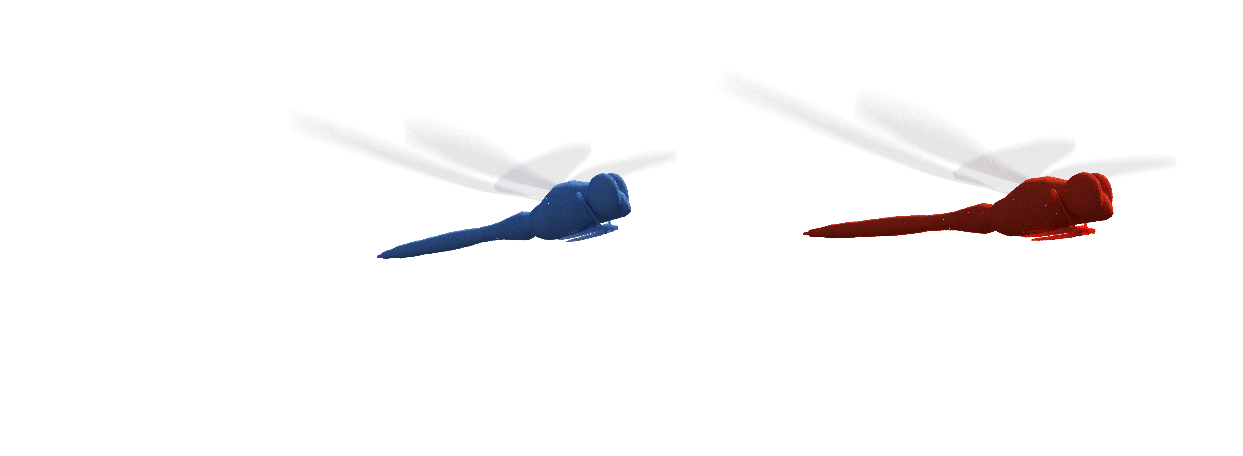
\includegraphics[height=.9\headerheight]{UPB_Logo_WEISS_12_libellen2.pdf}
}
%the poster title
{\color{white}\bf\smaller
  Sphere in a Box: \\ 
  Psychophysical experiments in \\ reality close context
}
%the author(s)
{\color{white}\small
\vspace*{-0.2cm}
  \vspace{1em}Alexander Kr{\"u}ger, Lukas Stratmann,  Ingrid Scharlau\\
  {\smaller alexander.krueger@uni-paderborn.de, lumpiluk@campus.uni-paderborn.de, ingrid.scharlau@uni-paderborn.de}
  
}


%%%%%%%%%%%%%%%%%%%%%%%%%%%%%%%%%%%%%%%%%%%%%%%%
% the actual content of the poster begins here
%%%%%%%%%%%%%%%%%%%%%%%%%%%%%%%%%%%%%%%%%%%%%%%%

\begin{posterbox}[name=intro,span=2,column=0,row=0]{Introduction}
\begin{tabular}{p{0.63\textwidth} p{0.3\textwidth}}
    Psychophysical experiments are designed to provide highly precise parameter estimations. Thus, numerous highly controlled trials are needed in an isolated enviroment. But due to this setting we lose realism, because in nativ environment we always have many confounding variables and a more complex visual stimulus.
    So our approach to get more reality close results is to embedd the experiment in a game-engine created  	surrounding with Unreal4.
    & 
    \vspace{-8pt}
    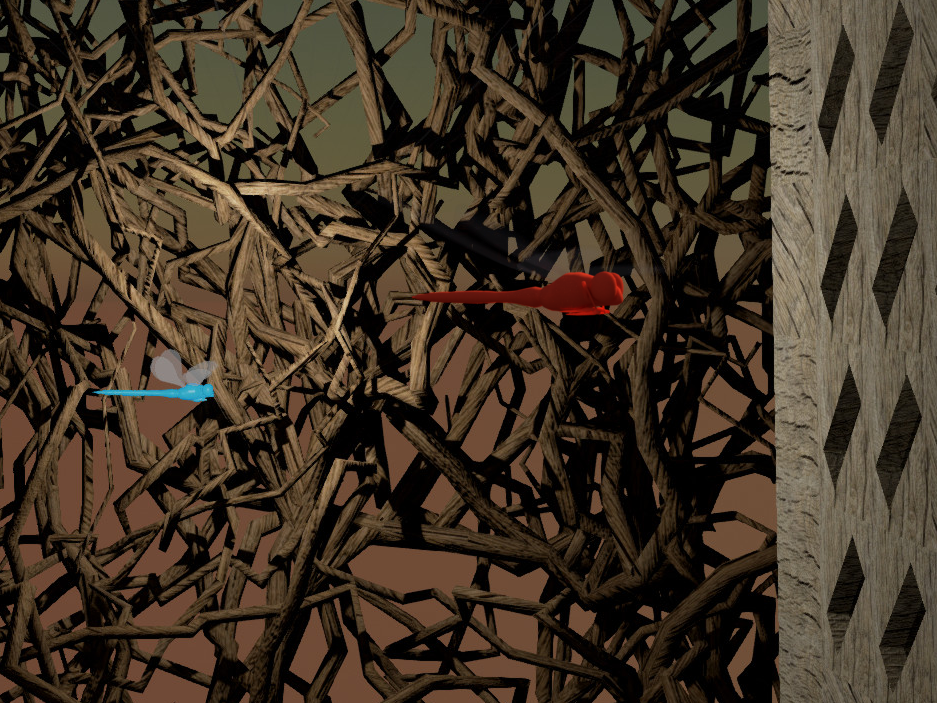
\includegraphics[width=0.32\textwidth]{race2.png}\\
\end{tabular}

\end{posterbox}

\begin{posterbox}[name=theory,column=0,row=1,below=intro]{Theory}
Visual attention can be understood as biased competition.
	\begin{itemize}
	\item stimuli ``race'' in parallel for brain's limited resources 
    \item competition is biased by relevance and visual contrast
	\end{itemize}
Bundesen's (1998) theory of visual attention (TVA) models this mathematically
	\begin{itemize}
	\item parameter \textcolor{deepskyblue}{C}, \textcolor{deepskyblue}{overall processing rate}, models available resources 
    \item parameter \textcolor{orangec}{w}, \textcolor{orangec}{attentional weight}, models attentional bias
	\end{itemize}
TVA can be applied to temporal-order judgments to measure attention (Krüger, Tünnermann, \& Scharlau, 2016)
	\begin{itemize}
	\item only two relevant stimuli for judgment (salient probe $p$, non-salient reference $r$)
    \item order judgment is interpreted as outcome of two TVA races at speed (rate) $v_p$ and $v_r$
	\end{itemize}
%\begin{tabular}{p{0.58\textwidth} p{0.38\textwidth}}
\begin{tabular}{p{0.52\textwidth} p{0.38\textwidth}}
\vspace{0cm} 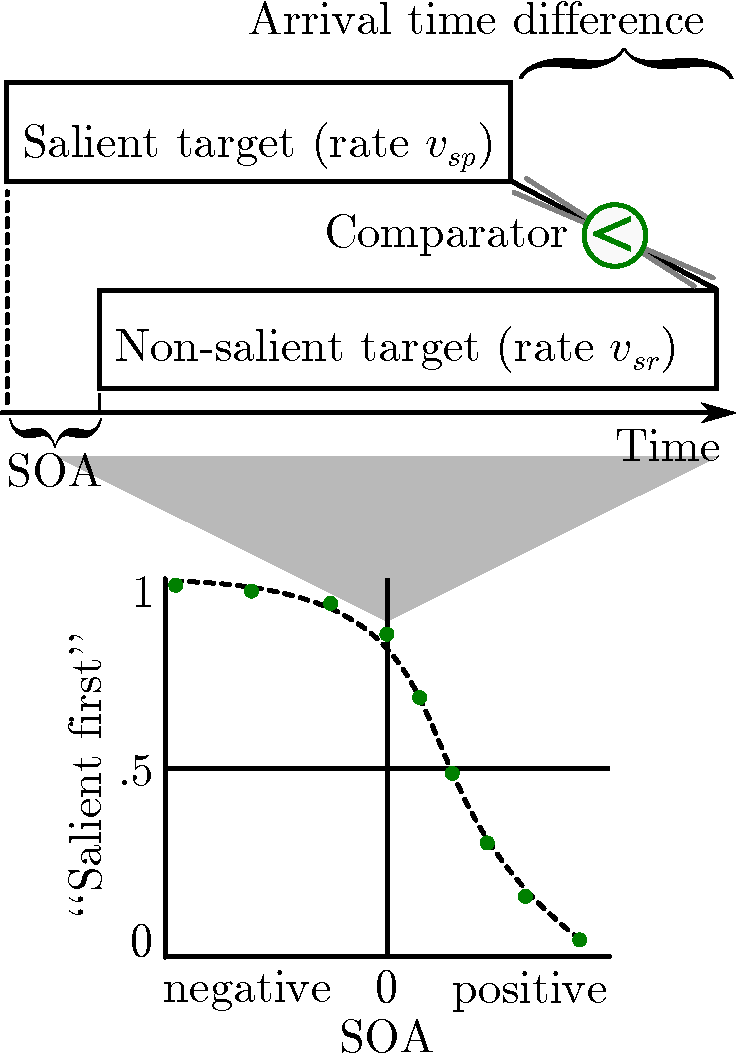
\includegraphics[width=0.485\textwidth]{imgs/cogmod.pdf} & \vspace{0cm}
$$v_p = \textcolor{orangec}{w_p} \cdot \textcolor{deepskyblue}{C}$$
$$v_r = w_r \cdot \textcolor{deepskyblue}{C}$$
$$w_r = 1-\textcolor{orangec}{w_p}$$
$$\textcolor{orangec}{w_p} =$$ 
$$ \kappa_p \sum_{j \in R} \eta(p,j)\pi_j$$ \\
\end{tabular}

The Game and the experiment measure \textcolor{orangec}{w}, \textcolor{orangec}{attentional weight}, and \textcolor{deepskyblue}{C}, \textcolor{deepskyblue}{overall processing rate}, from temporal-order judgments.
\end{posterbox}

\begin{posterbox}[name=game,span=1,column=1,row=1,below=intro]{Game}
\begin{itemize}
\item Dragonfly race through a pipe.
\end{itemize}
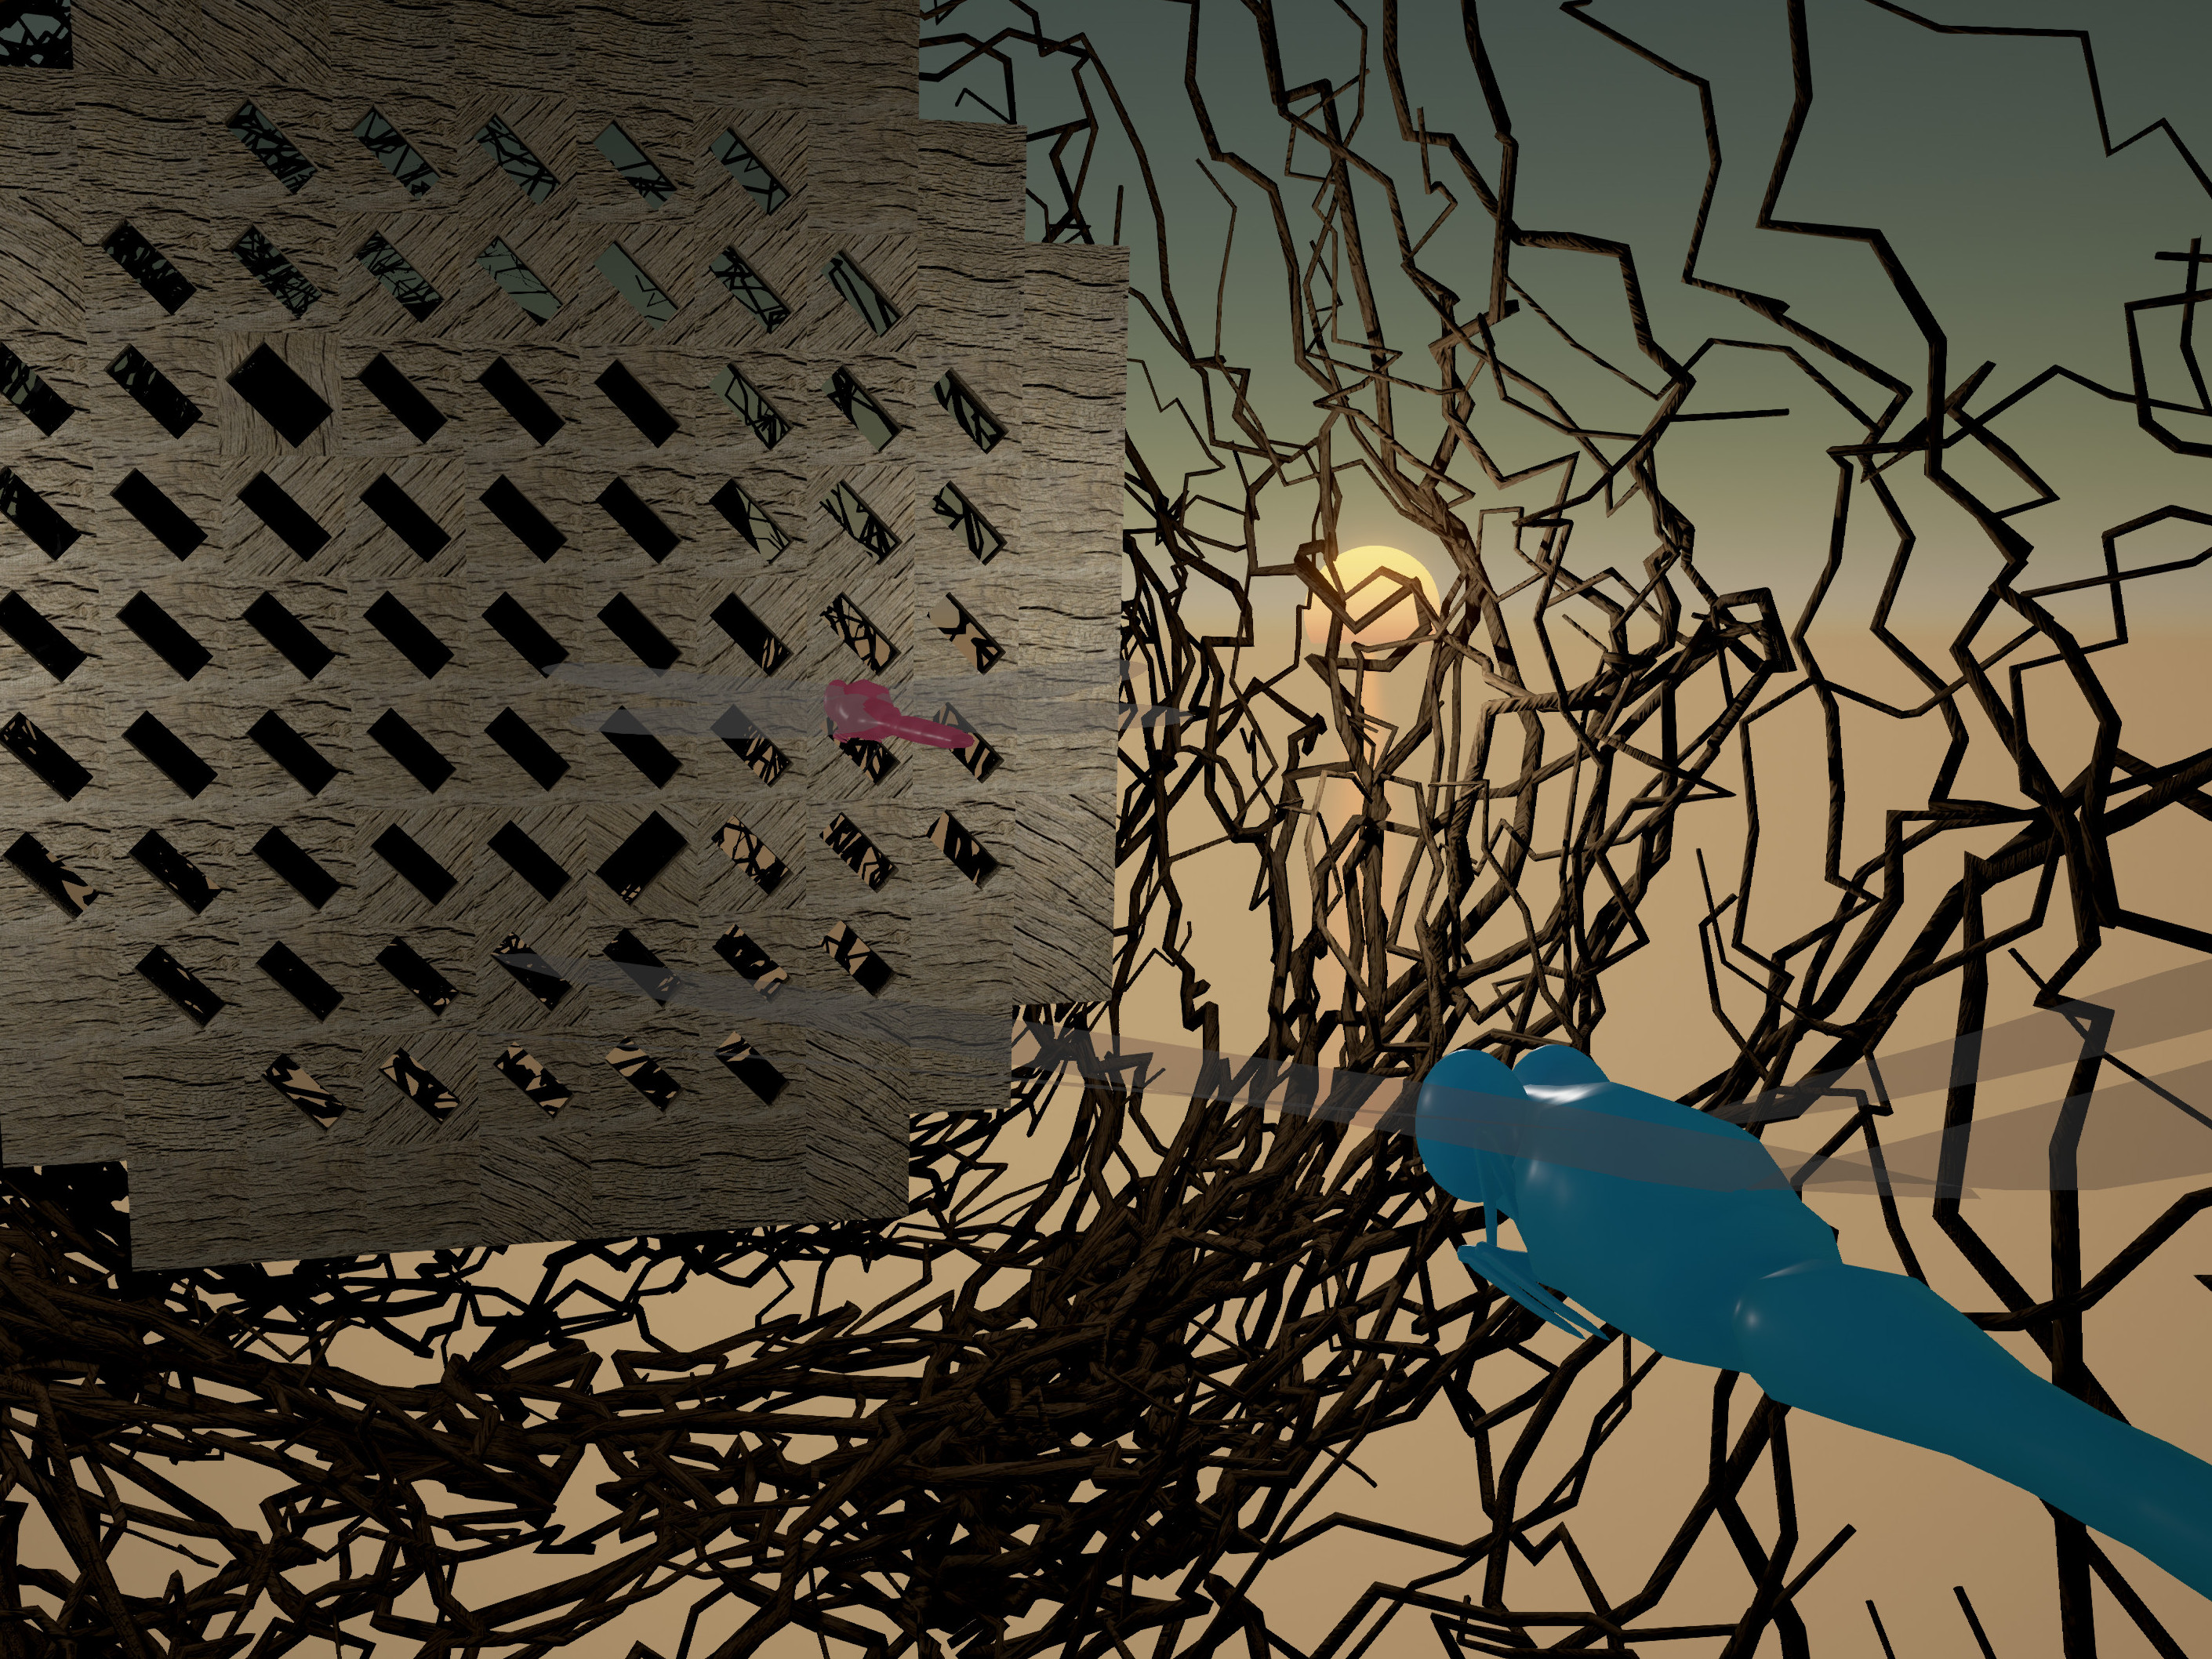
\includegraphics[width=1\textwidth]{game.jpg}
\begin{itemize}
\item Multiple grates obstruct the pipe.
\end{itemize}
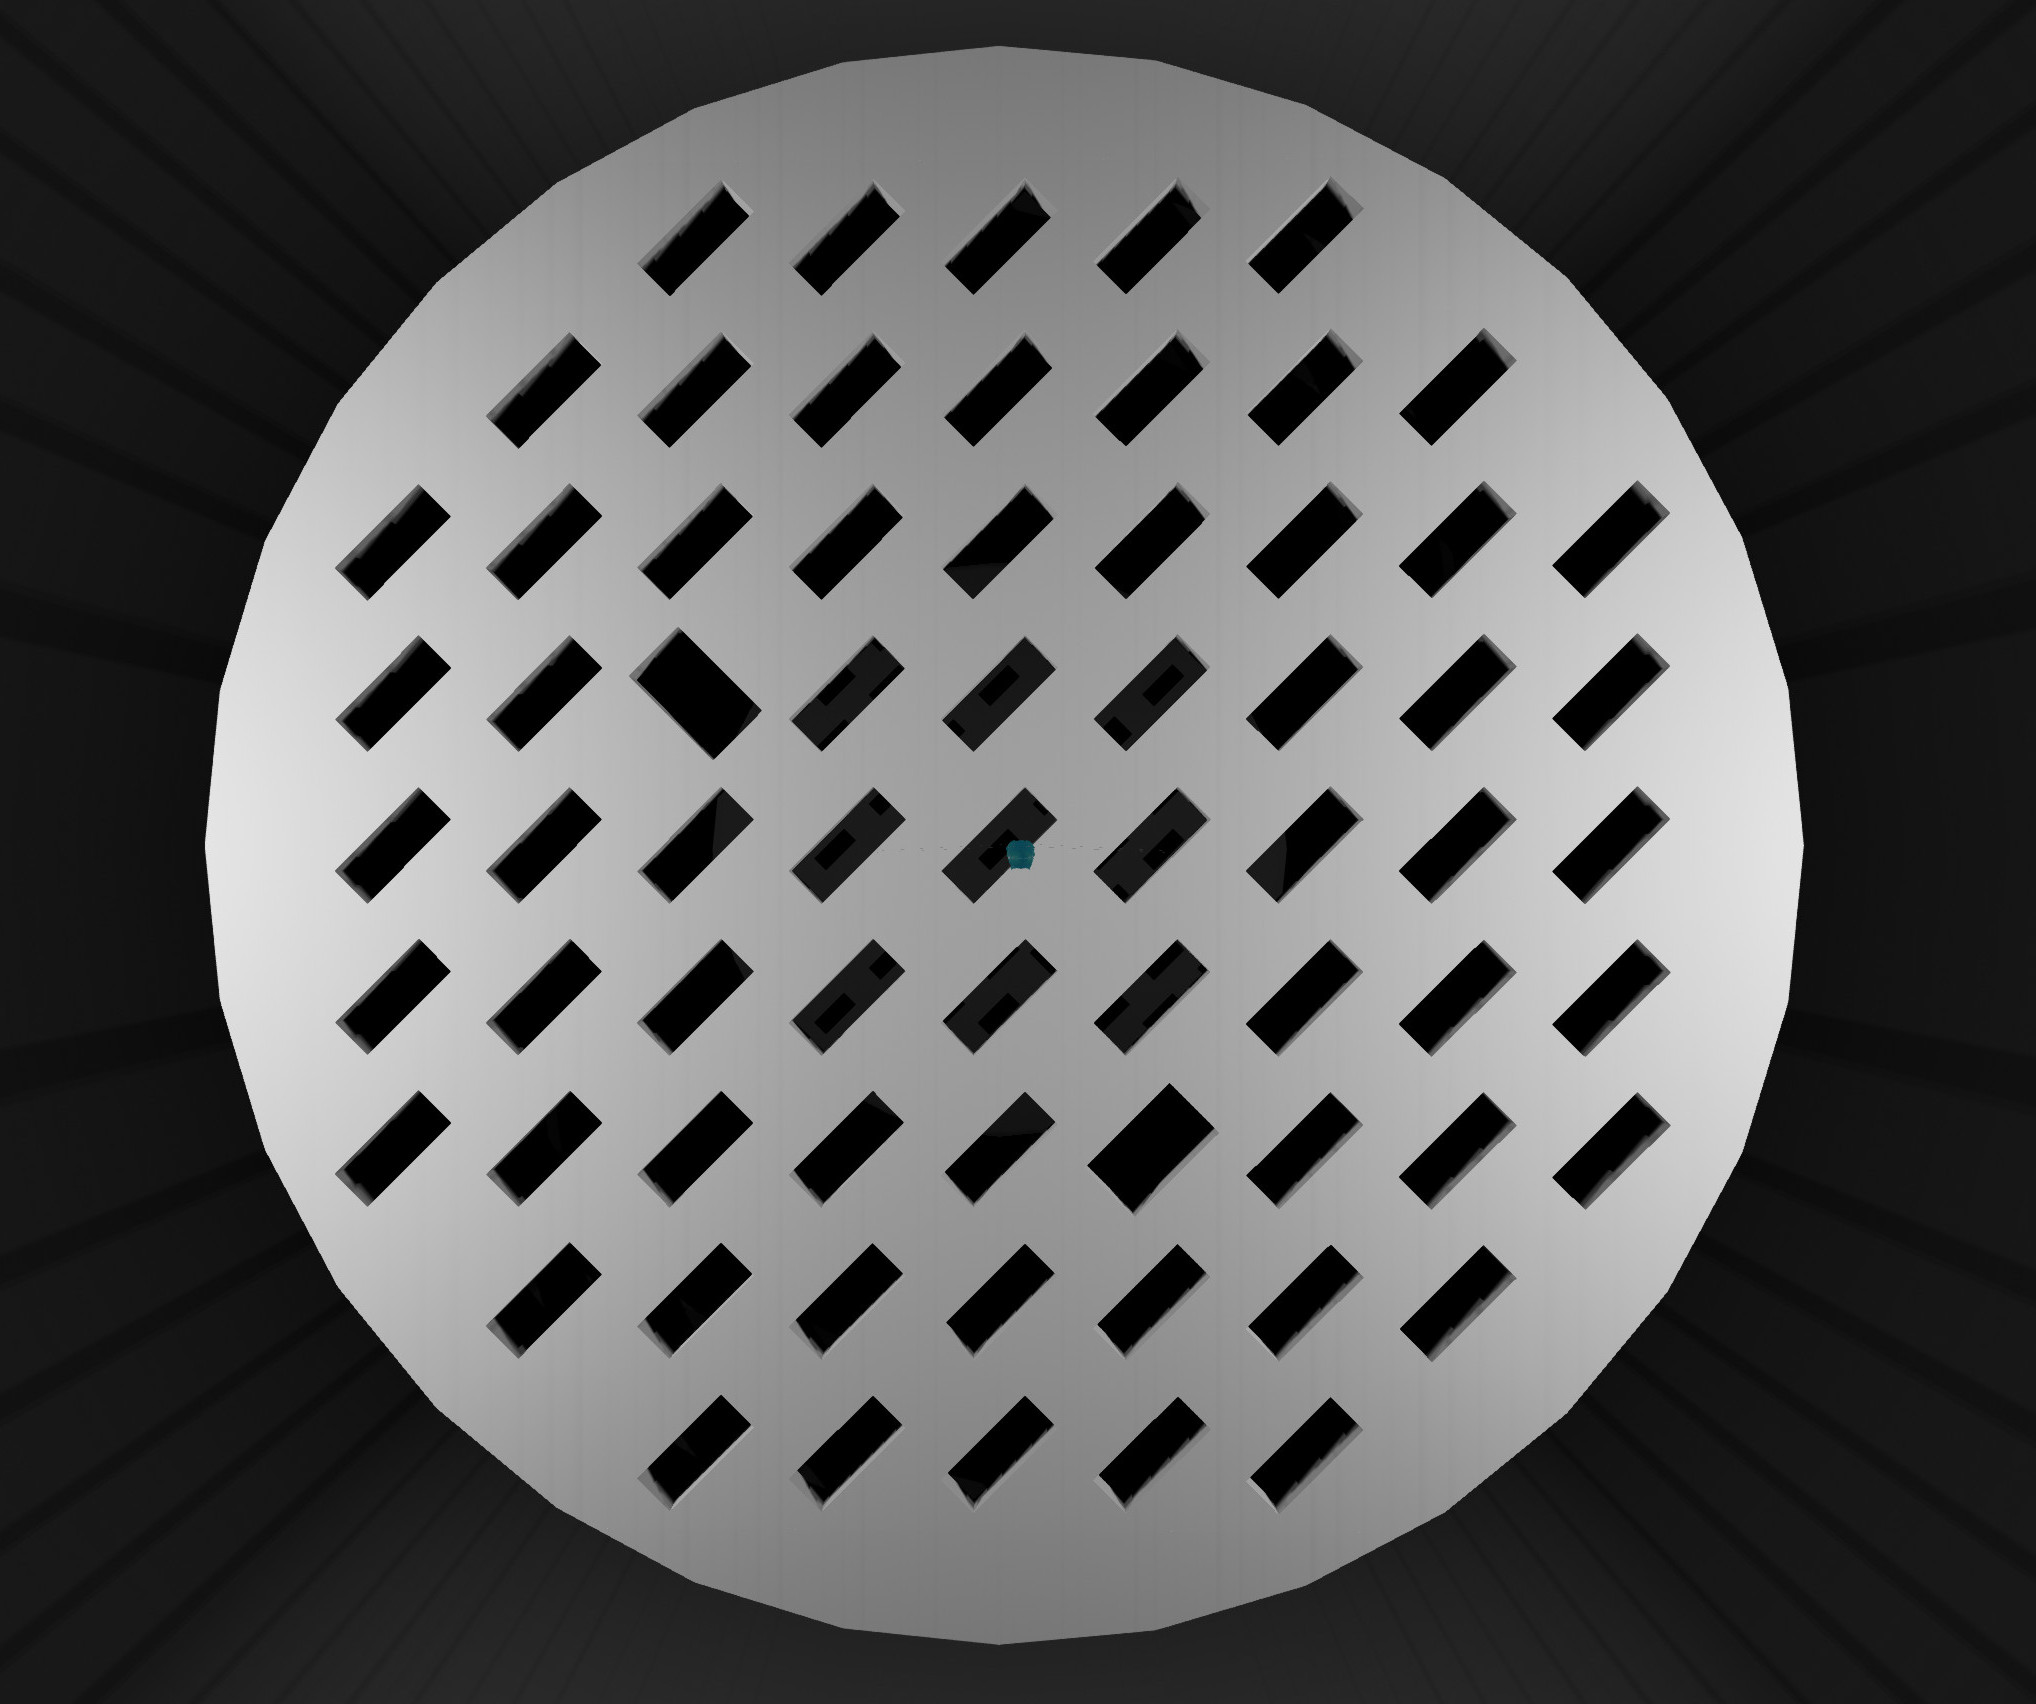
\includegraphics[width=1 \textwidth]{grate.jpg}
\begin{itemize}
\item Flying through two special openings provides bonuses.
\end{itemize}
\begin{itemize}
\item Discriminating their flicker correctly in time and flying through them accordingly increases bonus.
\end{itemize}
\end{posterbox}

\begin{posterbox}[name=procedure,span=2,column=0,row=2, below=game]{Procedure (game and classical experiment)}
\begin{center}
\includegraphics[width=0.85\textwidth]{procedurev2.pdf}
\end{center}
\end{posterbox}

\begin{posterbox}[name=results,span=1,column=2,row=0]{Analysis}
\begin{itemize}
\item Theory-based TVA parameters and data were connected by a Bayesian hierarchical model.
\end{itemize}
	\begin{center}
	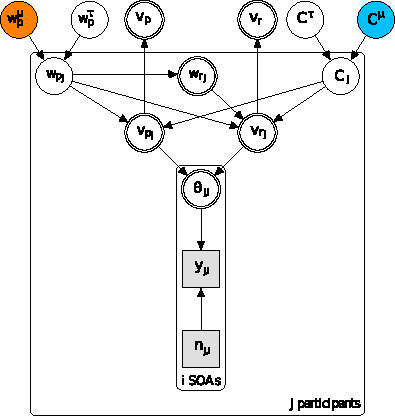
\includegraphics[width=0.5\textwidth]{graphmod.pdf}
	\end{center}
\begin{itemize}
\item Repetitions of trials per participant vary because of the freedom in the game -- difficult to model with classical statistics.
\end{itemize}

\begin{center}
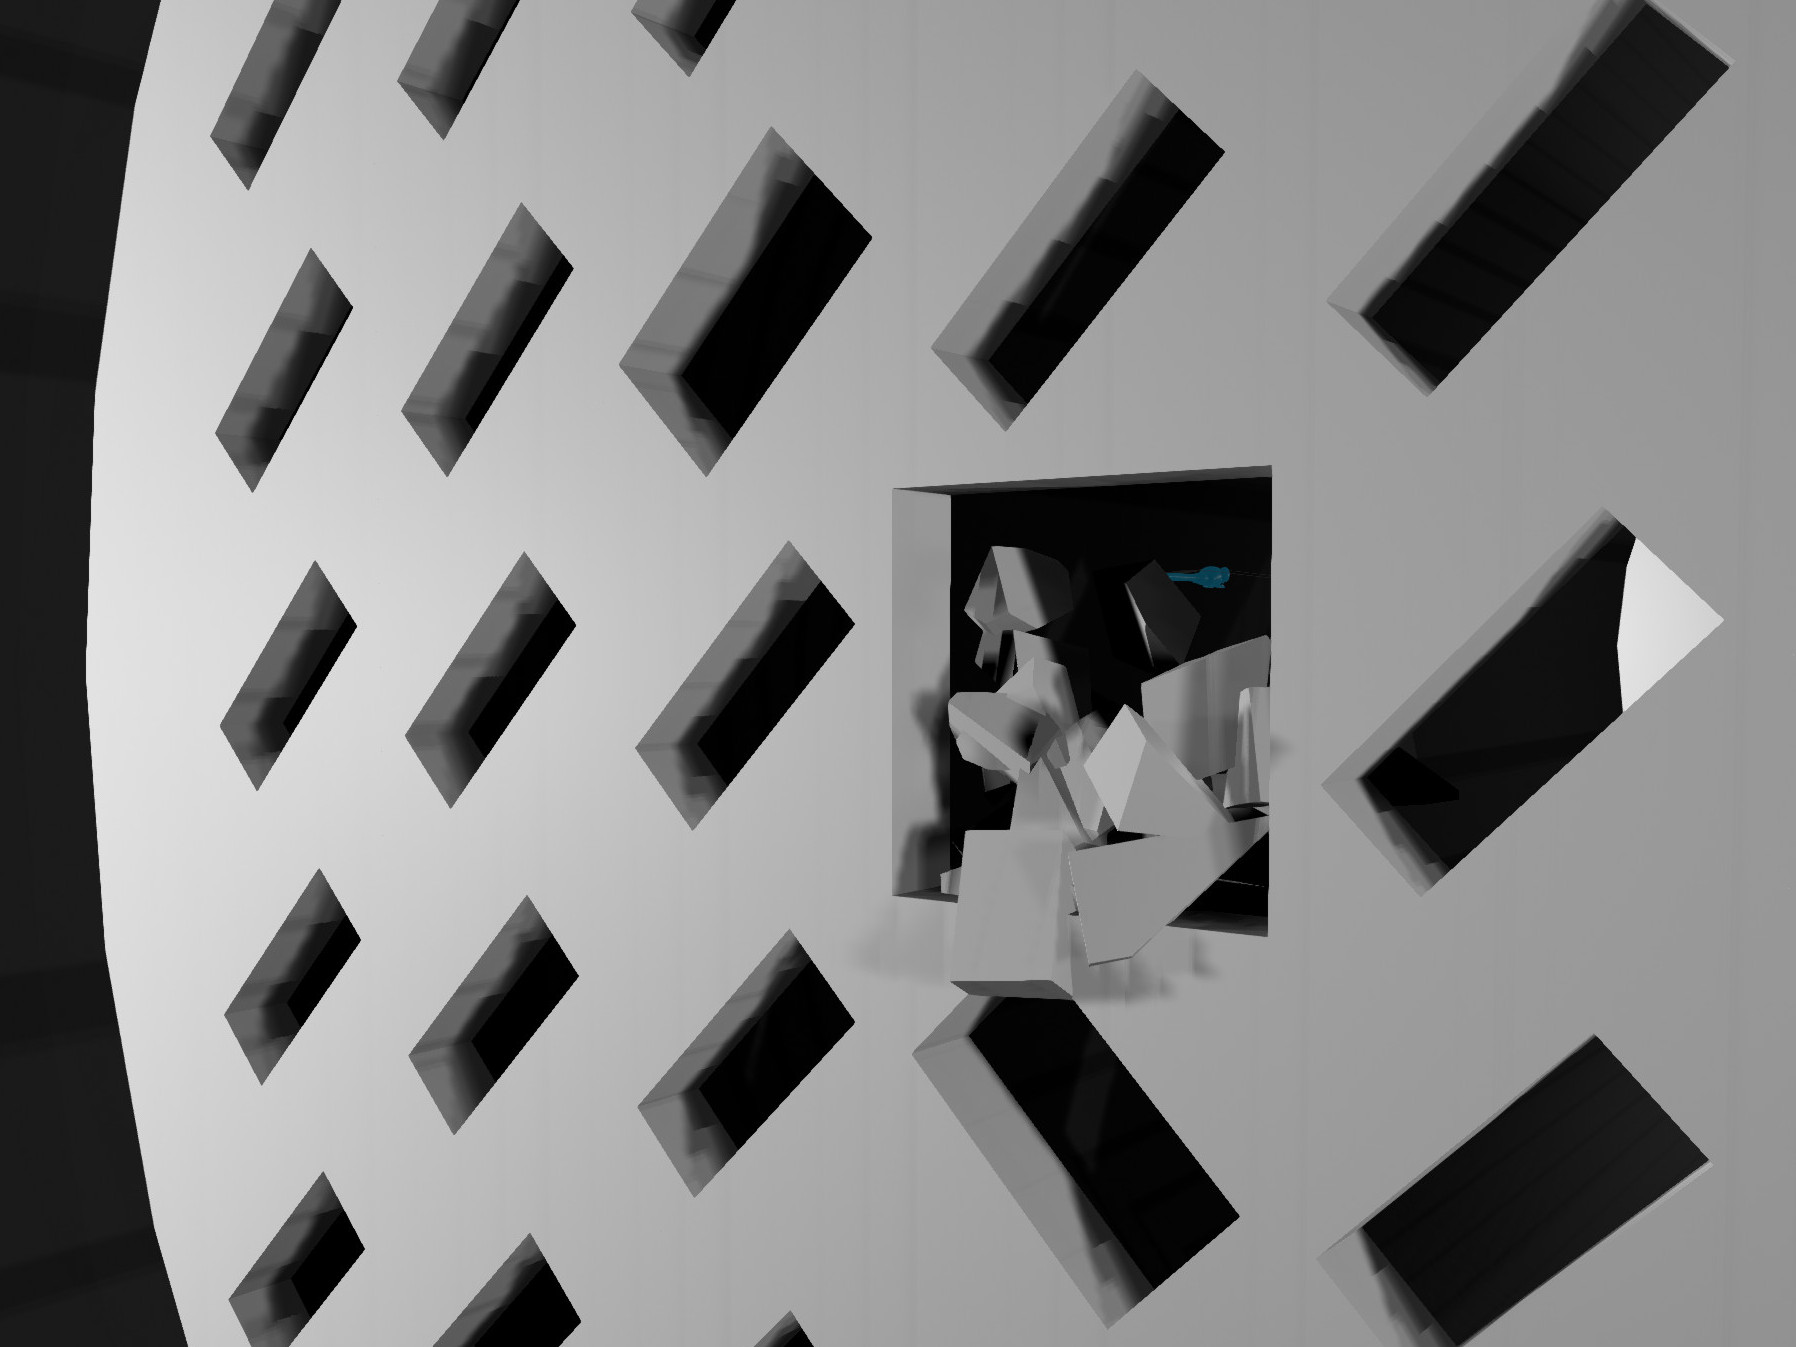
\includegraphics[width=0.48\textwidth]{unclear.jpg}
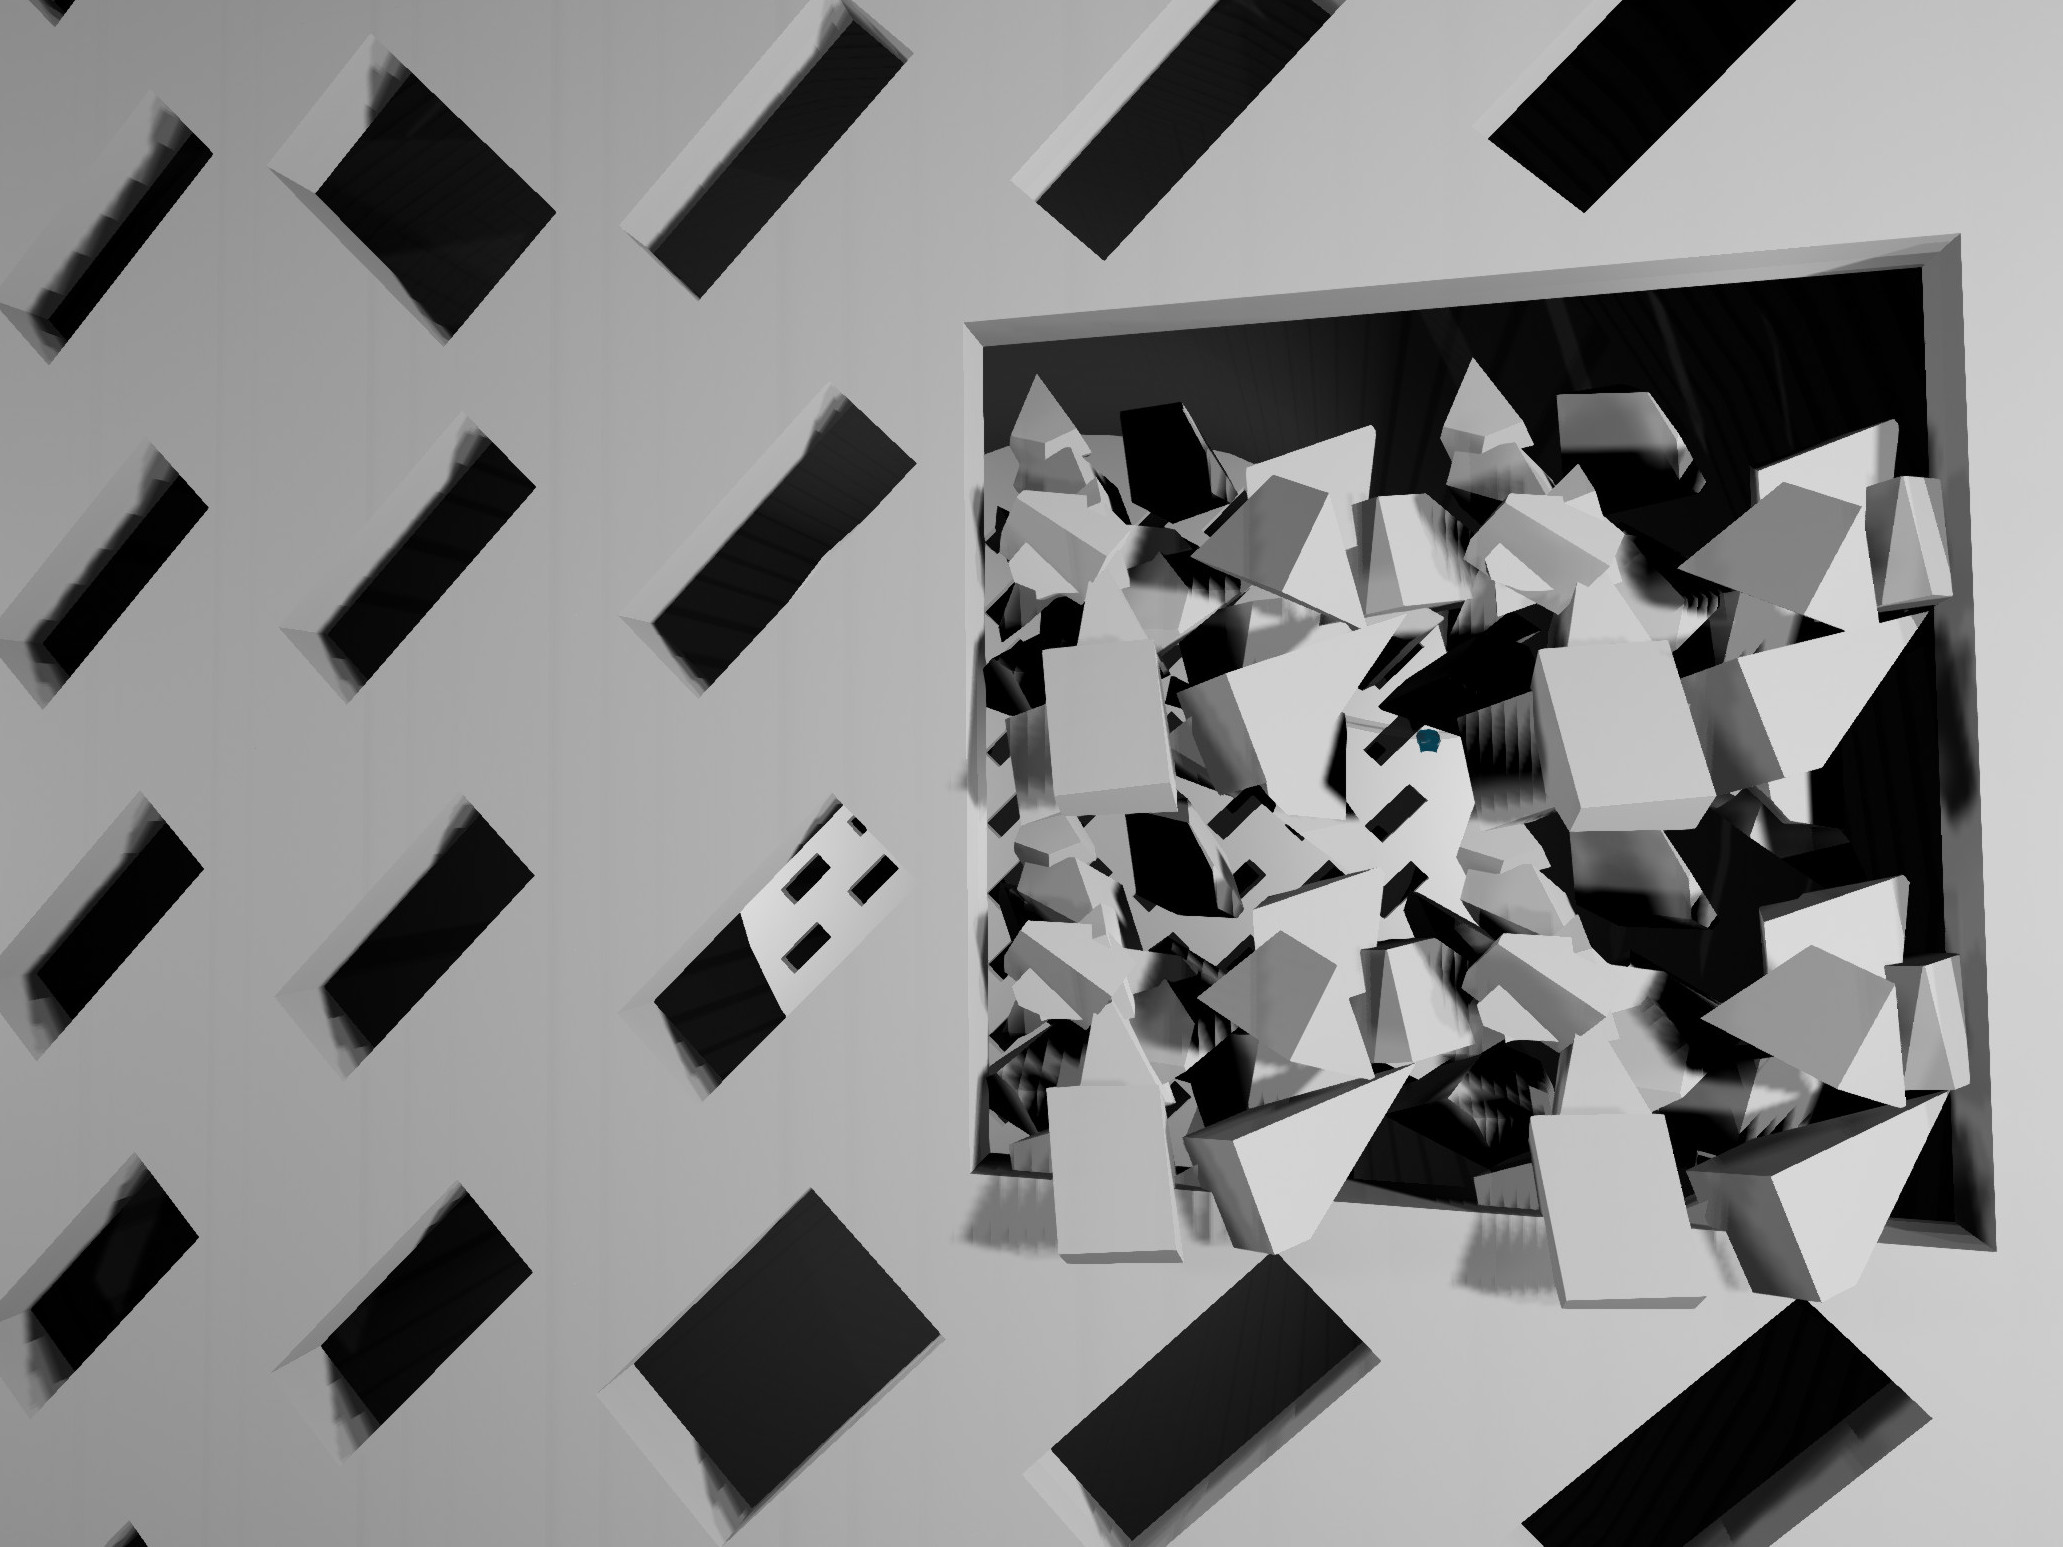
\includegraphics[width=0.48\textwidth]{unclear2.jpg}
\end{center}

\begin{itemize}
\item psychophysical parameter estimation: game (19 participants, ongoing)
\end{itemize}

\begin{center}
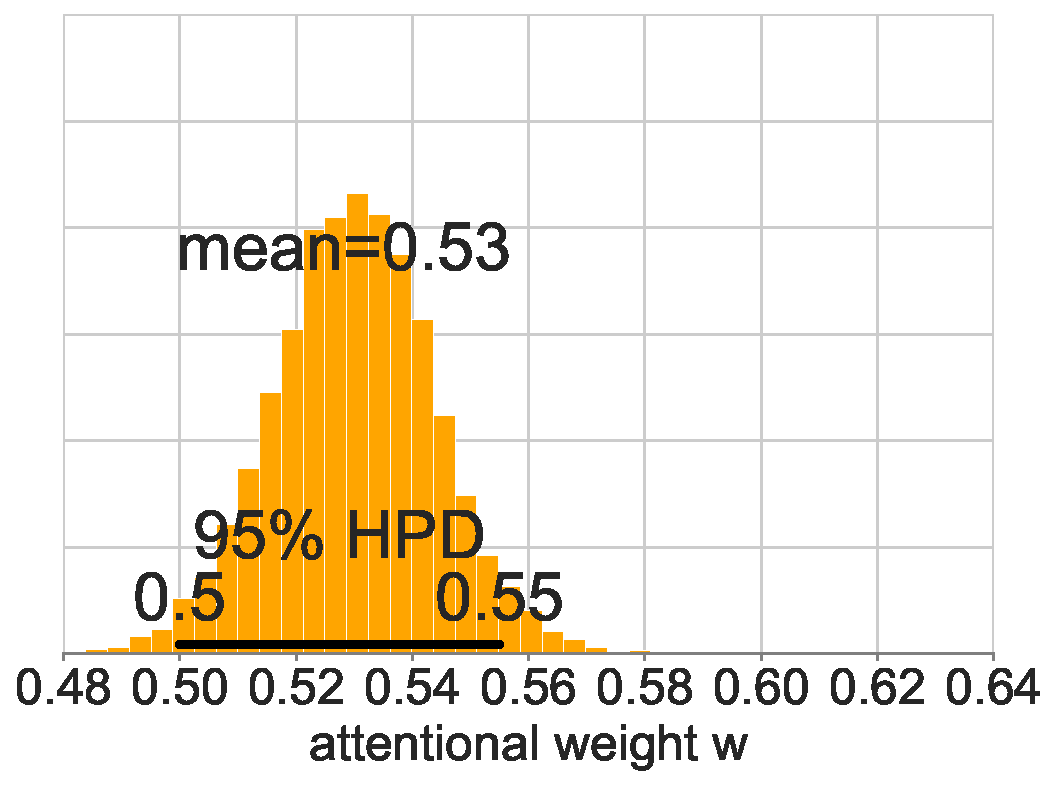
\includegraphics[width=0.48\textwidth]{game-w-hdi.pdf}
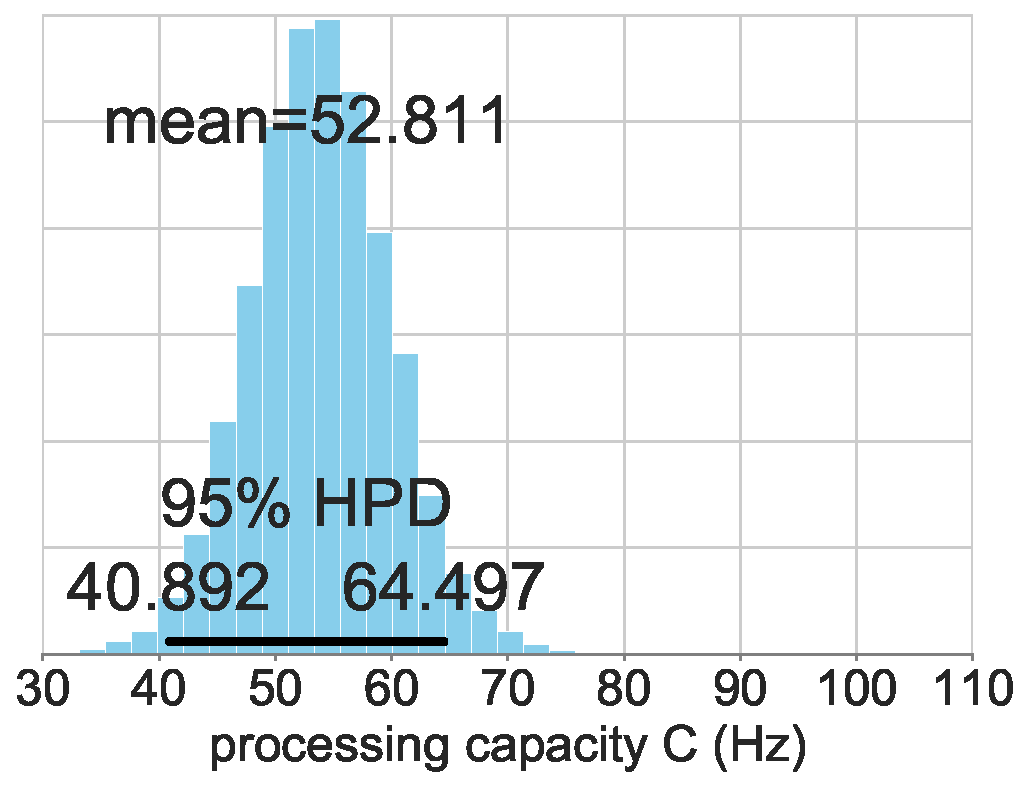
\includegraphics[width=0.48\textwidth]{game-c-hdi.pdf}
\end{center}

\begin{itemize}
\item psychophysical parameter estimation: classical experiment (13 participants, ongoing)
\end{itemize}

\begin{center}
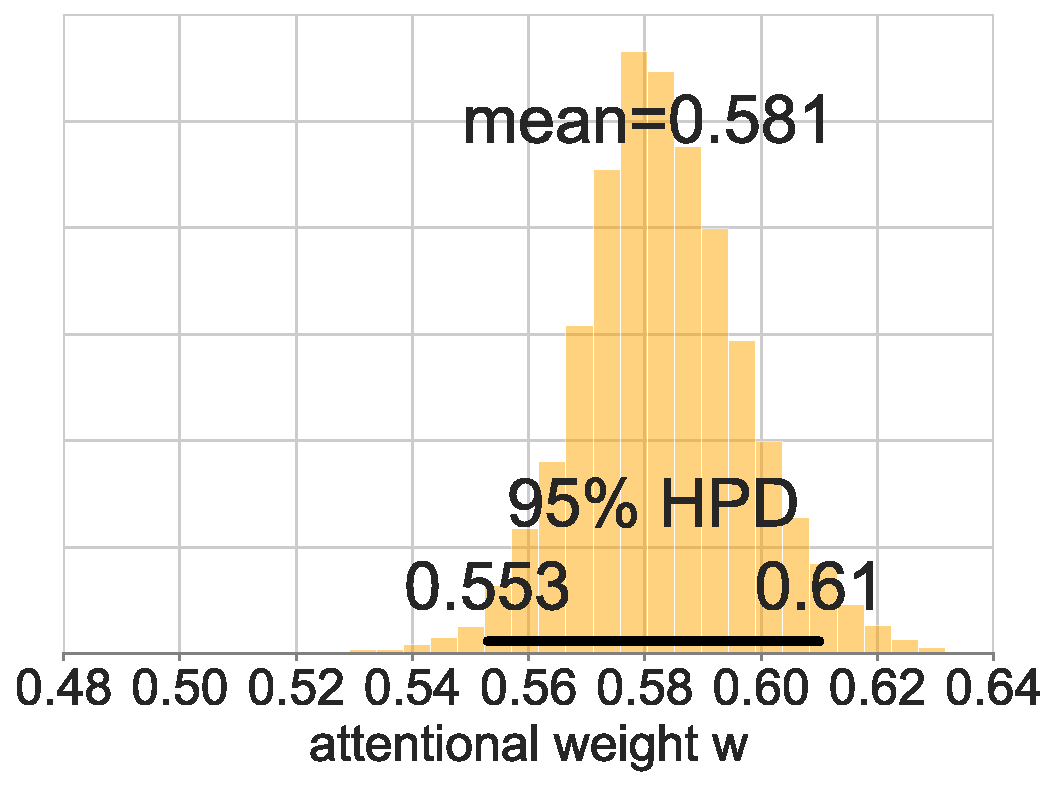
\includegraphics[width=0.48\textwidth]{exp-w-hdi-rs.pdf}
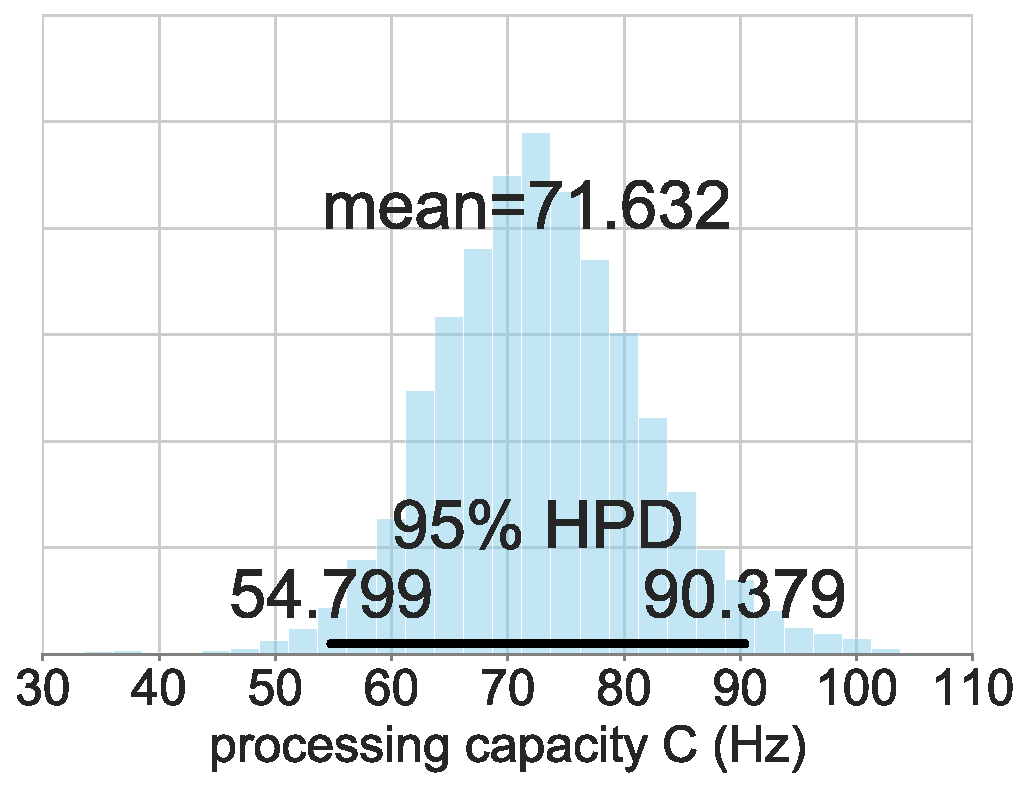
\includegraphics[width=0.48\textwidth]{exp-c-hdi-rs.pdf}
\end{center}

\end{posterbox}

\begin{posterbox}[name=conclusion,span=1,column=2,row=2,below=results]{Conclusion}
The results from the game and the classical experiment are similar: The salient probe stimulus receives an increased attentional weight in contrast to the reference stimulus. Importantly, estimation accuracy was comparable.

Quantitatively, there is a difference: In the game, the probe stimulus receives less attention and the overall visual processing capacity is reduced that may be caused by the necessity to visually monitor the position of the dragonfly. This requires capacity and attention to be distributed among three instead of two positions.

We conclude that the gaming approach is viable in general and that Bayesian data analysis allows for precise estimation despite the freedom in games.
\end{posterbox}

\begin{posterbox}[name=refs,column=0,span=3,below=procedure,above=bottom]{References}
\footnotesize
\linespread{1}

{\color{upbblue}Bundesen, C. } ({\color{upbblue}1998}). A computational theory of visual attention. \textit{Philosophical Transactions of the Royal Society of London B: Biological Sciences, 353, 1271-1281.}, doi: 10.1098/rstb.1998.0282 

{\color{upbblue}Krüger, A., Tünnermann, J., \& Scharlau, I.} ({\color{upbblue}2016}). Fast and conspicuous? Quantifying salience with the theory of visual attention \textit{Advances in Cognitive Psychology, 12(1), 20}, doi: 10.5709/acp-0184-1 
\vspace{0.115cm}
\end{posterbox}

\end{poster}
\end{document}